\section{Ergebnisse des Netzwerkes}
\label{sec:ergebnisse}
Das Model wurde nach dem Training auf den "Undersampling" Testdaten getestet.
Wir haben den "Undersampling" Satz genutzt, da wir vermeiden wollten doppelte Bilder im Testsatz zu haben.
Zudem brauchten wir eine Gleichverteilte Anzahl von Bilder pro Genre.
Der Testdatensatz hat so 78 Bilder pro Genre.
Mit dem genutzten Model konnten folgende Werte, auf den Testdaten, erziehlt werden
\begin{align*}
    \text{Genauigkeit} &= 48.18\, \% \\
    \text{Verlust} &= 2.36 \, .
\end{align*}
Um herauszufinden welche Genre am schlechtesten und am besten erkannt werden, haben wir zudem eine Konfusionsmatrix erstellt, welche in Abbildung \ref{fig:confusion} zu sehen ist.
\begin{figure}
    \centering
    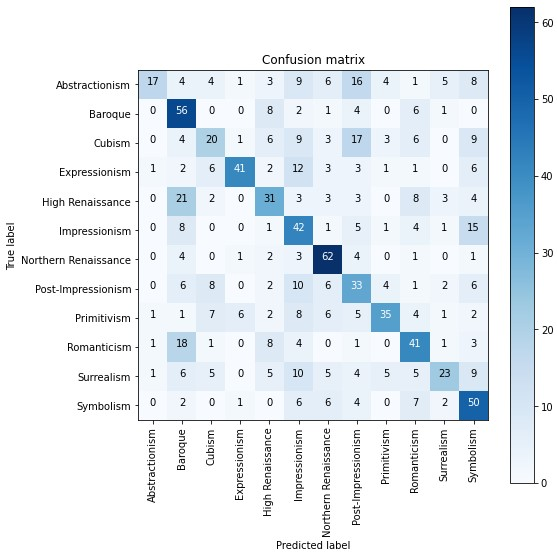
\includegraphics[width=0.5\textwidth]{content/data/confusion.JPG}
    \caption{Die Konfusionsmatrix zu den Testdaten mit dem genutzten Model.}
    \label{fig:confusion}
\end{figure}
Es lässt sich erkennen, dass besonders das Genre "Northern Renaissance" zu deutsch "Niederländische Renaissance" vom Model gut erkannt wird.
Dies ist damit zu begründen, das dieses Genre in dem genutzten Datensatz vorallem Bilder in schwarz-weiß enthält und so aus den anderen Bildern heraussticht.
Zudem verwechselt das Model am häufigsten "Hochrenaissance" Bilder (in der Abbildung mit "Highrenaissance" makiert) mit "Barock" Bilder (in der Abbildung mit "Baroque" makiert).
Wahrscheinlich liegt dies daran, dass beide Genre kräftige, kontrastreiche Farben nutzen und oft Menschen in Frontalansicht zeigen.
Um die falschen Vorhersagen des Models besser zu veranschaulichen wurden einige Bilder ausgegeben, dessen Genre falsch vom Model bestimmt wurden, diese sind in Abbildung \ref{fig:fehler} zu sehen.
Dabei steht "Predicted label" für die Vorhersagen des Models und "True label" für das wahre Genre des Bildes.
\begin{figure}
    \centering
    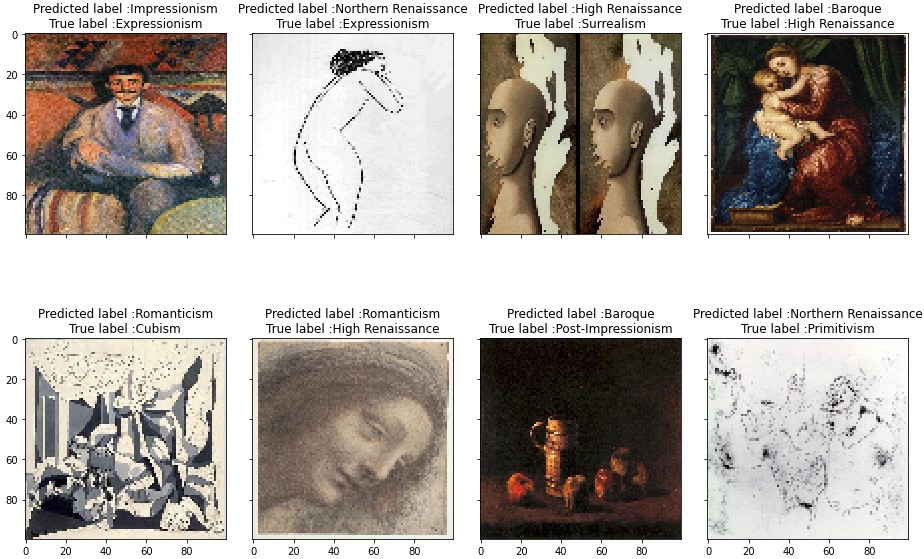
\includegraphics[width=\textwidth]{content/data/errors.JPG}
    \caption{Einige Bilder dessen Genre vom Model falsch bestimmt wurden.}
    \label{fig:fehler}
\end{figure}
Auch die falschen Vorhersagen sind bis auf einige Ausnahmen nachvollziehbar.
So sind in diesem Datensatz Bilder des Genre "Niederländische Renaissance" vor allem scharz-weiß, was die Abweichung in Bild 2 links oben und Bild 4 links unten erklärt.
Zudem ähnelt das Genre "Impressionismus" (in der Abbildung "Impressionism") von seiner Farbgebung und dem Stil sehr dem Expressionismus (in der Abbildung "Expressionism").
Wie bereits erwähnt nutzt das Genre "Hochrenaissance" (in der Abbildung mit "Highrenaissance" makiert) ähnliche Farben und Motive wie das Genre "Barock" (in der Abbildung mit "Baroque" makiert) wodurch die Verwechslung in dem Bild rechts oben zu begründen ist.
Die falsche Bestimmung des dritten Bildes von links oben kommt wahrscheinlich daher, dass in dem Bild ein menschlicher Kopf zu sehen ist, was ein typisches Motiv für die "Hochrenaissance" ist.
Woher die Abweichung der drei Bilder unten links stammen können wir allerdings nicht sicher sagen.